\section{Empirical Evaluation}
\label{evaluation}

We implemented our technique and used it to generate ca\-che-oblivious
divide-and-conquer implementations of three algorithms that were used as
benchmarks in \cite{IPDPS15/Tithi}, and a few others.

\begin{figure}[t!]
\vspace{-5mm}
\[
  \renewcommand\arraystretch{1.2}
  \begin{array}{@{}l@{}l@{}l@{}}
    \lspan3{w^x : ((I\times I)\cap{<})\to J\to\R} \\
    \lspan3{w^y : ((J\times J)\cap{<})\to I\to\R} \\
    G ~=~ \fix \theta\,i\,j\mapsto{}
      & \lspan2{\big[0\big]_{i=j=0} \,\Big/~ \big[w^y_{0j0}\big]_{i=0} \,\Big/~ \big[w^x_{0i0}\big]_{j=0} \,\Big/} \\
      & \min~\langle~ & \theta_{(i-1)(j-1)}+c_{ij}, \\
      & & \min p\mapsto\theta_{pj}+w^x_{pij}, \\
      & & \min q\mapsto\theta_{iq}+w^y_{qji} ~\rangle
  \end{array}
\]
\vspace{-3mm}
\caption{\label{evaluation:gap spec}
  Specifications for the Gap problem.}
\end{figure}

\begin{paragraph}{Parenthesis problem.} Our running example; Compute
an optimal placement of parentheses in a long chain of multiplication, e.g. of matrices, where the inputs
are cost functions $x_i$ for accessing the $i$-th element and
$w_{ikj}$ for multiplying elements $[i,k)$ by elements $[k,j)$.
\end{paragraph}

\begin{paragraph}{Gap problem.}
A generalized minimal edit distance problem. Given two input strings 
$\overline{x}=x_1\cdots x_m$ and $\overline{y}=y_1\cdots y_n$,
compute the cost of transforming $x$ into $y$ by any combination of the
following steps:
  (i) Replacing $x_i$ with $y_j$, at cost $c_{ij}$,
  (ii) Deleting $x_{p+1}\cdots x_q$, at cost $w^x_{pq}$,
  (iii) Inserting $y_{p+1}\cdots y_q$ in $\overline{x}$, at cost $w^y_{pq}$.
The corresponding recurrence is shown in \Cref{evaluation:gap spec}.
\end{paragraph}

\begin{paragraph}{Protein Accordion Folding problem.} A protein can be viewed
as a string $\mathcal{P}_{1..n}$ over an alphabet of amino acids. 
The protein folds itself in a way that minimizes potential energy.
Some of the acids are {\em hydrophobic}; minimization of the total hydrophobic
area exposed to water is a major driving force of the folding process.
One possible model is packing $\mathcal{P}$ in a two-dimensional square lattice
in a way that maximizes the number of pairs of hydrophobic elements,
where the shape of the fold is an {\em accordion}, alternating between going down and going
up.
\end{paragraph}

\medskip
We also exercised our system on a number of textbook problems:
the Longest Common Subsequence (LCS) problem, the Knapsack problem,
and the Bitonic Traveling Salesman problem.
\cbdelete\diffnote{\raggedright usability estimation moved to later}

\subsection{Implementation Details}
\cbstart\diffnote{separated implementation details from experiments}
The tactic application engine is implemented in Scala. We implemented a prototype
IDE using HTML5 and AngularJS, which communicates with the engine by sending
and receiving program terms serialized as JSON. Our system supports using either
Z3 or CVC4 as the back-end SMT solver for discharging proof obligations required
for soundness proofs. Synthesis of recursive calls is done by translating the
program to \Sketch{}, which solves a correct assignment to type parameters.
To argue for the feasibility of our system, we include
SMT solver running time for the verification of the three most used tactics (figures are for CVC4),
as well as time required for \Sketch{} synthesis, in \Cref{evaluation:solving time}.
We consider an average delay of \textasciitilde 10 seconds to be reasonable, even for an interactive
environment such as Bellmania.\cbend

Tactics are implemented as small Scala classes. It is possible for
the more advanced user to extend the library by writing such classes.
To give an idea, on top of the generic TAE the {\sf Stratify} tactic was coded in 12 lines of Scala,
including the functionality that breaks a function $h$ into two functions $f$ and $g$.

The compiler back-end is implemented as another component in
\cbstart\diffnoteup{\vspace{-1cm}as part of AE, the compiler back-end was ported to Scala}Scala\cbend, processing ASTs and generating C++ code containing Intel Cilk constructs for parallelization.
It employs a thin intermediate representation layer at which the optimizations of \Cref{codegen} are applied.

\cbstart\diffnote{separated implementation details from experiments}\vspace{-1em}% the neg vspace is only needed because of \marginpar (introduced by \diffnote)
\subsection{Experimental Results}
\label{evaluation:experimental}
\cbend

Table~\ref{evaluation:cppruntimes} shows performance improvement for our 
auto-generated implementation (AUTO) on the state-of-the-art optimized parallel
loop implementation (LOOPDP) from~\cite{IPDPS15/Tithi}. It also compares AUTO with manually 
optimized recursive implementations CO\_Opt and COZ for the three problems from~\cite{IPDPS15/Tithi}. 
Our compiler automatically does \textit{copy optimization} 
as done in CO\_Opt and COZ. COZ also incorporates a low-level 
optimization of using Z-order layout of the array,
which is out of scope for this paper. %pointer arithmetics for loop traversal? 
%Explicit vectorization of loops?
$N$ is the problem size and $B$ is the base case size for using loops 
instead of recursion. It can be seen from the table that our \cbdelete\diffnote{removed remark about further optimizing by hand} implementation 
performs close to the manually optimized code.
Figure~\ref{fig:gap} depicts the performance of these implementations on one sample instance
as a function of problem size, and shows the scalability of the generated code. 

\begin{table}
\centering
\renewcommand\a{({\it i})}    % relax! it's only for this figure
\renewcommand\b{({\it ii})}
\renewcommand\c{({\it iii})}
\begin{tabular}{|l|rr@{\quad}r@{\quad}|r@{\quad}|}
  \cline{2-5}
  \multicolumn{1}{c|}{} & \multicolumn{3}{c|}{\small Verification} & \multicolumn{1}{@{\,}c@{\,}|}{\small Synthesis} \\
  \multicolumn{1}{c|}{} & \multicolumn{1}{c|}{\sf Slice} & \multicolumn{1}{c|}{\sf Stratify} & \multicolumn{1}{c|}{\sf Synth} & \multicolumn{1}{c|}{Sketch} \\
  \hline
  {\bf Paren               }  &  0.9  &  8.7   &   0.9  &  24.5     \\
  \hline
  {\bf Gap                 }  &  0.6  &  6.8   &   1.4  &  11.6     \\
  \hline
  {\bf Protein             }  &  0.9  &  3.8   &   0.7  &  9.5     \\
  \hline
  {\bf LCS                 }  &  0.9  &  1.9   &   0.5  &  3.2     \\
  \hline
  {\bf Knapsack            }  &  0.3  &  1.9   &   0.4  &  5.3     \\
  \hline
  {\bf Bitonic             }  &  0.9  &  7.2   &   0.6  &  10.1     \\
  \hline
\end{tabular}
\caption{\label{evaluation:solving time}
  Average proof search time for proof obligations and average synthesis
  time for {\sf Synth} parameters (seconds).}
\end{table}



\begin{table}
\centering
\begin{tabular}{|l|c|c|c|c|}
    \cline{2-5}
  \multicolumn{1}{c|}{} & \multicolumn{4}{c|}{\scriptsize Speedup w.r.t parallel LOOPDP on 6 cores}  \\
  \multicolumn{1}{c|}{} & \multicolumn{4}{c|}{\scriptsize   CPU (12 workers), B=64}  \\
  \multicolumn{1}{c|}{} & \multicolumn{1}{c|}{~~N~~} & \multicolumn{1}{c|}{CO\_Opt} & \multicolumn{1}{c|}{~~COZ~~} & \multicolumn{1}{c|}{AUTO}  \\
  \hline
  {\bf Parenthesis}  & 16384  & 32x & 50x & 46x\\
  \hline
  {\bf Gap}  & 16384 & 21x & 34x & 30x\\
  \hline
  {\bf Protein} & 16384  & 2.2x & 2.6x & 1.4x \\
  \hline
  {\bf LCS}  & 45000 & $-$ & $-$ & 1.5x \\
  \hline
  %{\bf Knapsack} & $-$ & $-$ & ?x\\
  %\hline
  {\bf Bitonic}  & 45000  & $-$ & $-$ & 4.2x\\
  \hline
\end{tabular}
\caption{\label{evaluation:cppruntimes}
  Performance of different C++ implementations}
\end{table}

\begin{figure}
\resizebox{8cm}{!}{
\begin{tikzpicture}[>=latex,mark options={scale=.5}]
	\begin{axis}[
	    ymode=log,
		xlabel=Problem size,
		ylabel=Time ({\it s}),
		scaled x ticks=false, %{real:1000}
		log basis y=2, ymajorgrids=true]
	\addplot[color=blue!50!white,ultra thick,mark=*,smooth] table[x=n/Time(s),y=COZ] {data/perf-gap.txt}
	  node(COZ-curve) [coordinate,pos=0.9] {};
	\addplot[color=orange!70!white,ultra thick,mark=*,smooth] table[x=n/Time(s),y=CO] {data/perf-gap.txt}
	  node(CO-curve) [coordinate,pos=0.8] {};
	\addplot[color=olive!70!white,ultra thick,mark=*,smooth] table[x=n/Time(s),y=LOOPDP] {data/perf-gap.txt}
	  [yshift=-12pt] node[pos=0.05] {LOOPDP};
	\addplot[color=red!70!white,ultra thick,mark=*,smooth] table[x=n/Time(s),y=Bellmania] {data/perf-gap.txt}
	  node(Bellmania-curve) [coordinate,pos=0.85] {};
	\end{axis}
	
	\begin{scope}[anchor=west]
	  \node(CO-lbl)[orange!80!white] at(2,1.5) {CO\_Opt};
	  \node(Bellmania-lbl)[red!80!white] at(1.5,1) {Bellmania};
	  \node(COZ-lbl)[blue!80!white] at(1.25,.5) {COZ};
	\end{scope}
	\begin{scope}[->,dashed]
	  \draw[orange] (CO-lbl) -- (CO-curve);
	  \draw[red] (Bellmania-lbl) -- (Bellmania-curve);
	  \draw[blue] (COZ-lbl) -- (COZ-curve);
	\end{scope}
\end{tikzpicture}

}
\caption{\label{fig:gap} Performance comparison for parallelized implementations for Gap problem on 6-core Intel i7 CPU}
\end{figure}

\newcommand\isum[1]{\pgfmathparse{int(#1)}\pgfmathresult}

\begin{table}
\centering
\begin{tabular}{|l|r@{\quad}r@{\quad}|r@{\quad}|}
  \cline{2-4}
  \multicolumn{1}{c|}{} & \multicolumn{2}{c|}{\small Conceptual} & \multicolumn{1}{c|}{\small Bellmania} \\
  \multicolumn{1}{c|}{} & \multicolumn{1}{c}{\# phases} & \multicolumn{1}{c|}{\# steps} & \multicolumn{1}{c|}{\# tactics} \\
  \hline
  {\bf Paren               }  &   3   &   \isum{4 + 9 + 9}   &   \isum{4 + 14 + 12}   \\
  \hline
  {\bf Gap                 }  &   3   &   \isum{9 + 9 + 9}   &   \isum{19 + 17 + 17}  \\
  \hline
  {\bf Protein             }  &   4   &   \isum{5 + 7 + 7 + 9}  &   \isum{10 + 11 + 12 + 14} \\
  \hline
  {\bf LCS                 }  &   1   &   5             &   5   \\
  \hline
  {\bf Knapsack            }  &   2   &    \isum{7 + 9} &   \isum{25 + 24}       \\
  \hline
  {\bf Bitonic             }  &   3   &    \isum{5 + 5 + 6} &   \isum{11 + 10 + 11}  \\
  \hline
\end{tabular}
\caption{\label{evaluation:user effort}
  Sizes of synthesis scripts compared to conceptual problem size (see \Cref{evaluation:effort}).}
\end{table}

\subsubsection{Estimation of User Effort}
\label{evaluation:effort}

Because Bellmania is an interactive system, we try to give a measure as to how much effort a typical user has to invest
to complete a development for the DP algorithms that comprise our test suite.
To get an idea of how domain experts think about the problem, we consult~\cite{PPoPP16/Chowdhury},
where descriptions are conveniently provided in the form of data-flow diagrams for each step of computation.
An example for such a diagram, corresponding to our \Cref{overview:recursive-A}, is shown in \Cref{evaluation:par-A-diag}; in this case, we count it as 4 steps.

%\pagebreak
%\begingroup  % want to do it but causes fig to move to the end :/
\setlength{\columnsep}{3mm}% anyway it's too late for \columnsep to affect anything at this point
\setlength{\intextsep}{3mm}
%
\begin{wrapfigure}{r}{2.8cm}
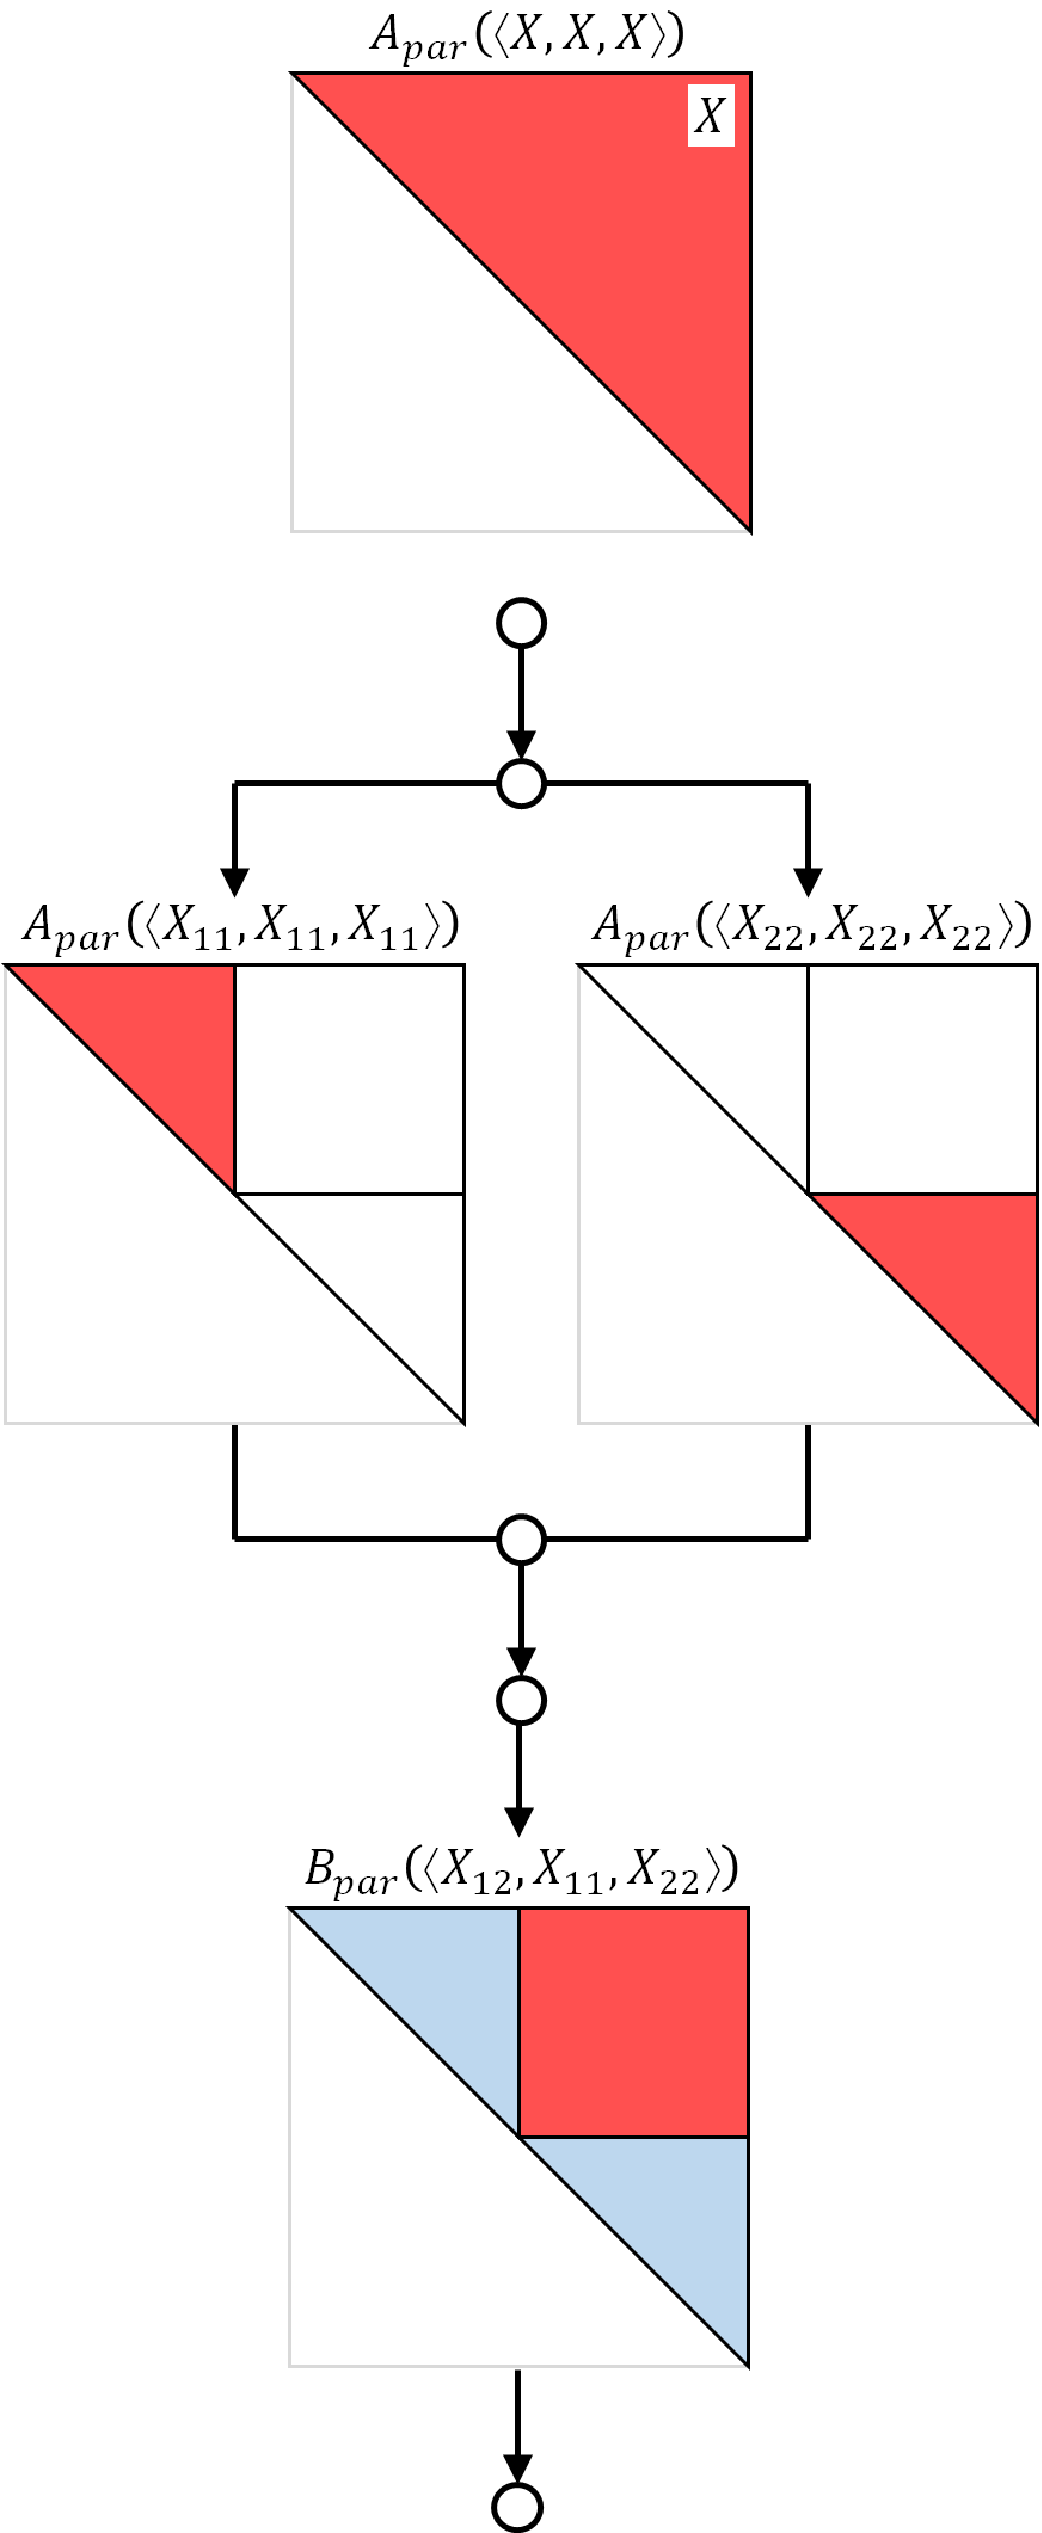
\includegraphics[width=.15\textwidth,trim=0mm 0mm 2mm 0mm]{img/par-A.pdf}
\caption[An example diagram]{\label{evaluation:par-A-diag}\\
  An example \\diagram (from~\cite{PPoPP16/Chowdhury})}
\end{wrapfigure}
%
%\endgroup

\cbstart\diffnote{\vspace{2mm}explained the numbers, and admitted the need for a more thorough study}%
We compare the sizes of these diagrams, which we label ``\# steps'', with the number of tactic
applications required to derive the respective implementation in Bellmania.
The results of the comparison are given in \Cref{evaluation:user effort}, where ``\# phases''
indicates how many recursive subroutines are included in the algorithm description 
(and in the respective development) and the two other columns give the sizes of the description vs. that of the development.
The development size is within $2\times$ of the diagrams' size in most cases, peaking at $3\times$.

Diagrams and complete Bellmania transcript for the running example are included in \Cref{annex:example:paren}.

Admittedly, the measured volume ratio provides a crude proxy for usability.
A controlled user study should be run to provide true evidence,
but that goes beyond the scope of this paper.
Still, the results are reassuring since through the course of developing the
tool we were able to reduce the number of reasoning steps from hundreds to
a few dozens, and also make them high-level.
We were also able to detect mistakes in existing (hand written) formulations
of divide-and-conquer algorithms, that eluded discovery by experts.
The additional examples in the appendix and the in accompanying technical report
should furnish sufficient intuition to conceive a qualitative opinion on
the efficacy of the approach and the prototype.
\cbend

%~\\~  % waste to lines to get to the end of the wrapfig
% (\vspace doesn't work because wrapfig only counts actual lines)
